\documentclass{LeanTestReport}
\usepackage{wrapfig}
\usepackage[titles]{tocloft} % modify ToC 
\usepackage{lipsum}
\usepackage{float} % better placement of figures with 'H'
\cftsetindents{section}{0em}{3em} 
\cftsetindents{subsection}{0em}{3em}
\cftsetindents{subsubsection}{0em}{4em}
\renewcommand{\arraystretch}{1.2} % to add extra space between the rows

\definecolor{customcolor}{HTML}{2287BA}
\definecolor{litecustomcolor}{HTML}{E6F4FF}

\fancyhf{}
\fancyhead{%
\begin{minipage}[t]{1.0\linewidth}%
  \begin{minipage}{0.4\linewidth}%
    
\includegraphics[scale=0.18]{dummyLogo}%
  \end{minipage}%
  \begin{minipage}{0.6\linewidth}%
    \begin{flushright}%
      Full Name \\
      \url{https://www.example.com} \\
      jane.doe@example.com \\
    \end{flushright}%
  \end{minipage}%
  \vspace{0.1cm}~\\%
\vspace{0.4cm}\noindent\makebox[\linewidth]{\rule{\linewidth}{0.4pt}}\noindent%
\end{minipage}%
}
% Footer
\rfoot{Page \thepage\ of \pageref{LastPage}} 

% First page style change
\fancypagestyle{first}{%
  \fancyhf{}
  \rfoot{Page \thepage\ of \pageref{LastPage}}
}
\fancypagestyle{firstNoF}{\fancyhf{}}

\begin{document}
\pageOneMargins
\thispagestyle{first}
% \thispagestyle{firstNoF} % uncomment to remove footer

\setlength{\leftskip}{-0.2in} % counter minipage ofset 
\begin{minipage}[t]{0.55\linewidth}


\begin{minipage}{0.4\linewidth}%
    \vspace{0.08in}%
    
\includegraphics[scale=0.18]{dummyLogo}%
  \end{minipage}%
  \begin{minipage}{0.6\linewidth}%
    \begin{flushright}%
    Full Name \\
    \url{https://www.example.com} \\
    jane.doe@example.com \\
    \end{flushright}
  \end{minipage}
\vspace{-0.3cm}~\\
\vspace{0.4cm}\noindent\makebox[\linewidth]{\rule{\linewidth}{0.4pt}}
\noindent%

%%%%%%%%%
%  START OF THE PAGE 1 Main Column (do not overfill height, continue on page 2)
%%%%%%%%%

\begin{center}
{\LARGE Example Testing Project}\\
\today \\
\end{center} 
\vspace{0.35 cm}
Organization Name \\
Organization Address Line One \\
Organization Address Line Two \\
\url{https://www.example.com}

\vspace{0cm}\noindent\makebox[\linewidth]{\rule{\linewidth}{0.4pt}}

\section*{Executive Summary}

\lipsum[1-2]

\section*{Source Code References}

%\begin{small}
\begin{flushleft}
\href{https://www.github.com/github/}{Example Repository One:}
\\
\href{https://www.github.com/github/}{https://www.github.com/github/}
\medskip
 
\href{https://www.github.com/ndebuhr/}{Example Repository Two:}
\\
\href{https://www.github.com/ndebuhr/}{https://www.github.com/ndebuhr/}
\medskip 

\end{flushleft}

%\end{small}


%%%%%%%%%
%  START OF THE Side Column
%%%%%%%%%
\end{minipage} \hspace{0.25in}%
\begin{minipage}[t]{0.4\linewidth}
\vspace{-0.24in}
\begin{mybox}
\textbf{Status:}\\
Completed, Awaiting Approval
\end{mybox}

\subsection*{Key Results}

\begin{center}
\rule{\textwidth}{1pt}%
\vspace{0.22in}
Key Metric One \\
\section*{XX.XX \%}
\rule{\textwidth}{1pt}%
\vspace{0.22in}
Key Metric Two \\
\section*{XX,XXX Users}
\rule{\textwidth}{1pt}%
\vspace{0.22in}
Key Metric Three \\
\section*{XXX ms}
\rule{\textwidth}{1pt}
\end{center}

\vfill
\end{minipage}
\newpage
\setlength{\leftskip}{0in} % back to normal after minipage ofset
\restoregeometry % back to normal header margins

%%%%%%%%%
%  START OF THE PAGE 2
%%%%%%%%%

\section*{Raw Data}

\lipsum[1]

\begin{figure}[H]
\centering
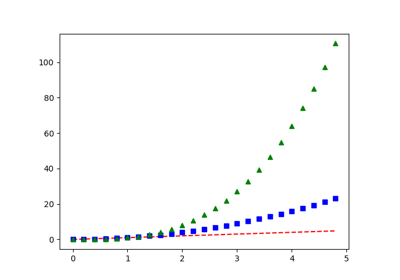
\includegraphics[width=0.7\textwidth]{examplePlot}
\caption{Example Plot}
\end{figure}

\lipsum[1-2]

\begin{figure}[H]
\centering
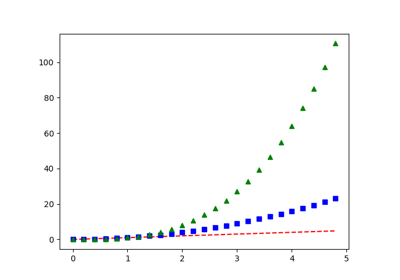
\includegraphics[width=0.7\textwidth]{examplePlot}
\caption{Example Plot}
\end{figure}

\begin{figure}[H]
\centering
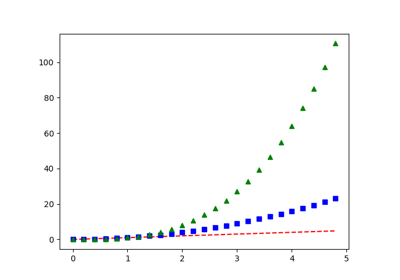
\includegraphics[width=0.7\textwidth]{examplePlot}
\caption{Example Plot}
\end{figure}

\begin{figure}[H]
\centering
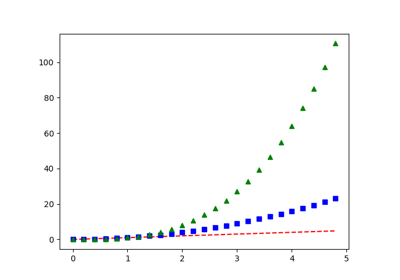
\includegraphics[width=0.7\textwidth]{examplePlot}
\caption{Example Plot}
\end{figure}

\section*{Discussion}

\lipsum[6-9]

\section*{Additional Information}

\lipsum[10]

\end{document}
